\chapter[Motivation of the experiment]{Motivation of the experiment}
\label{chap:motivation}

The accelerating gradient profile in a travelling-wave cavity depends from the configuration of the electromagnetic field inside. The passage of the  beam modifies the internal field configuration. As consequence, the gradient profile gets modified and results lower at the end of the structure.

At the same input power, the modification of the gradient profile is dependent from the beam current, as shown in Fig. \ref{grad_vs_I}. The result of the beam loading of the cavity is a reduction of the average accelerating gradient.

\begin{figure}[h]
\centering 
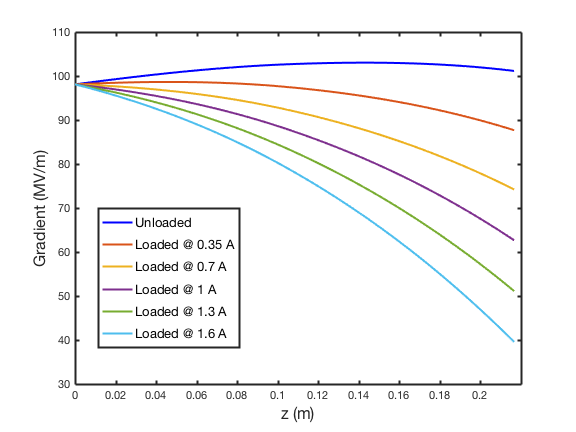
\includegraphics[scale=0.5]{pictures/Gradient_vs_current.png}
\caption{Gradient profile along the TD26CC structure at 43.3 MW input power. The unloaded case and the loaded with different current intensities are shown. The average gradient difference between the following curves is approximately 5 MV/m.}
\label{grad_vs_I}
\end{figure}

\noindent
The particle energy gain is given by 
\begin{equation}
\Delta W  = q \int_0^L E_{\text{acc}} (z) \, dz = q \left \langle E_{\text{acc}} \right \rangle L
\label{en_gain}
\end{equation}
where the q is the charge, E$_{\text{acc}}$ is the accelerating field and L the length of the accelerating structure.

Equation \ref{en_gain} shows that the energy gain is reduced when the accelerating cavity is loaded with the beam, compared to the unloaded condition. To compare the tests carried out without beam with the real running condition in an accelerator, it becomes necessary to raise the input power when the beam is present, in order to compensate the loss of average accelerating gradient. The nominal parameters for CLIC are 1.2 A of beam current and 100 MV/m of loaded accelerating gradient \cite{CLIC:cdr}. Figure \ref{100mvm} shows the variation of the gradient profile between loaded and unloaded running condition for the CLIC nominal operation. In this case the input power has to be raised from~43.3 MW to 61.3~MW to maintain the average accelerating gradient to 100 MV/m (see Table~\ref{TD26_param_1}).

\begin{figure}[h]
\centering 
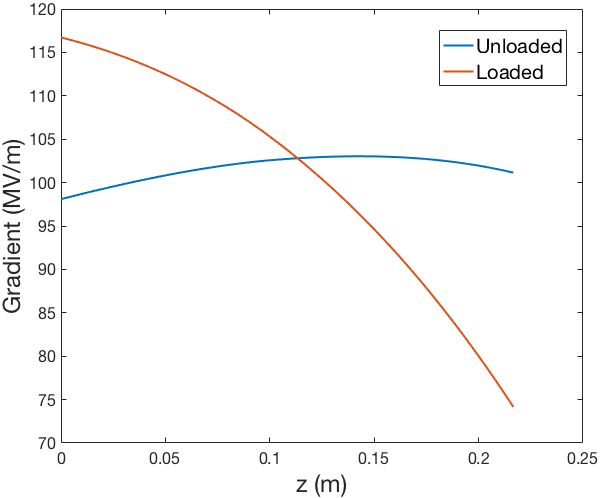
\includegraphics[scale=0.45]{pictures/grad_vs_IP.png}
\caption{Comparison of the loaded and unloaded gradient profile of the TD26CC structure loaded with the CLIC Main Beam. When loaded with a current of 1.2 A , the input power to maintain the 100 MV/m of average gradient pass from 43.3 MW of the unloaded case to the 61.3 MW for the loaded case. }
\label{100mvm}
\end{figure}

The breakdown rate tests are always conduced without the beam inside, and the vacuum arc phenomenon is not supported yet from a solid physical theory. For these reasons there is no way to predict a priori how the breakdown rate is affected from the presence of the beam. The first dedicated experiment and its results will be described in this work.

As comparison, the interesting measurements that can be carried out are:
\begin{enumerate}
\item Comparing measurements loaded and unloaded at the same input power
\item Comparing measurements loaded and unloaded at the same average gradient
\item Studying the effect of the antiloading, i.e. the beam deceleration due to the wrong relative phase between beam and RF
\end{enumerate}
regarding the last point, it has to be noted that the behaviour of the gradient profile in the antiloaded condition is the opposite of the loaded one. This is coming from the fact that the beam is releasing energy in the cavity in the form of RF during the slowing down process. The comparison of the three running conditions is shown in figure \ref{3grad}

\begin{figure}[h]
\centering 
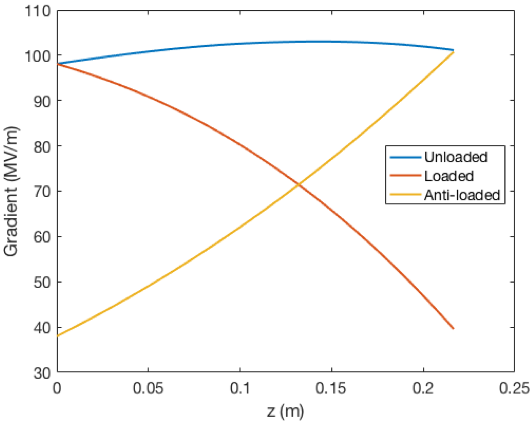
\includegraphics[scale=1]{pictures/3gradient.png}
\caption{Comparison of gradient profiles in different running conditions. The loaded and unloaded profiles are calculated at 43.3 MW input power, the antiloaded at 6.5 MW input power. }
\label{3grad}
\end{figure}